% !TEX encoding = UTF-8 Unicode
\documentclass[12pt]{article}
%\usepackage[utf8x]{inputenc}
%\documentclass[conference]{IEEEtran}

%\usepackage[latin1]{inputenc}
%\usepackage[portuguese]{babel}
\usepackage[brazil]{babel}
\usepackage[T1]{fontenc}
\usepackage[utf8x]{inputenc}

%\usepackage[alf]{abntcite}
\usepackage[alf]{abntex2cite}
%\usepackage[none]{hyphenat}
\usepackage[pdftex]{graphicx}
\usepackage{subfigure}
\usepackage[cmex10]{amsmath}
%\usepackage[dvips]{pstricks}
\usepackage{pst-all}
\usepackage{cite}
\usepackage{sbc-template}
%\usepackage{pst-plot}x
\hyphenation{FLAMAC}
%\usepackage{pst-plot}x

\newcommand{\meunome}{Hugo Vinícius Vaz Braga}
\newcommand{\meutitulo}{Camadas de Acesso ao Meio para Redes de Sensores Sem Fio}
\newcommand{\meuano}{2011}
\newcommand{\meuorientador}{Orientador: Prof. Flávio Assis}

%%%%%%%%%%%%%%%%%%%%%%%%%%%%%%%%%%%%%%%%%%%%%%%%%%%%

%% O comando \obs aqui definido permite que o autor faca anotacoes na
%% monografia que aparecem no PDF gerado. Para ativar o comando, descomente
%% a primeira linha e comente a segunda.
%% Exemplo de uso: \obs{Preciso melhorar este parágrafo...}

%\newcommand{\obs}[1]{\underline{\textbf{OBSERVAÇÃO}}: \emph{#1}}
\newcommand{\obs}[1]{}

\def\ordfem{\mbox{\raise .35em \hbox{\underline{\scriptsize a}\ }}}
\def\ordmasc{\mbox{\raise .35em \hbox{\underline{\scriptsize o}\ }}}
\def\prof{Prof\ordmasc.}

\begin{document}
% !TEX encoding = UTF-8 Unicode
% Capa com Brasão

\begin{titlepage}
   \begin{center}
    	%logotipo
               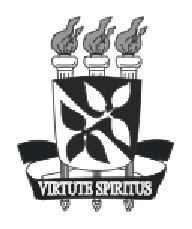
\includegraphics{imagens/brasaoUFBA} \\
	%\vspace{0.7in}
              \centering{ 
	      \bf{
	      \LARGE{
		\uppercase{UNIVERSIDADE FEDERAL DA BAHIA} \\
 	      }
	      \Large {
                   	\uppercase{Especialização Avançada em Sistemas Distribuídos} \\
	      }
              } }
   \end{center}
   \vfill
   \begin{center}
       \bf{
       \large{\uppercase{\meunome}  \\  }
       }
   \end{center}
   \vspace{0.2in}
   \begin{center}
       \bf{
      	 \LARGE{ \uppercase{\meutitulo} } \\
         \obs{\\ \Large{Esta versão da monografia contém comentários do autor.
          Para removê-los, redefina o comando LaTeX \texttt{obs}.}}
       }
   \end{center}

   \vfill
   \hspace{\stretch{1}}
   \vfill
   \begin{center}
      \normalsize{
          Salvador \\
          \meuano
       }
   \end{center}

\end{titlepage}

%comando abaixo cria uma capa redundante, mas como a capa com brasão foi 
% feita 'manualmente', não faz sentido usar este comando:
%\capa


% !TEX encoding = UTF-8 Unicode

%\folhaderosto
% o comando acima foi comentado para não criar uma folha de 
% rosto redundante, já que ela feita 'manualmente' abaixo

\begin{titlepage}
 \vfill
 \begin{center}
   {\large \uppercase{ \bf{ \meunome\ } } } \\[7cm]
   {\Huge \uppercase{ \bf{ \meutitulo\ } } }\\[1cm]
   \vfill
   \hspace{.45\textwidth} % posicionando a minipage
   \begin{minipage}{.5\textwidth}
     %\begin{espacosimples}
       \bf{
	Texto em formato de artigo apresentado ao Curso de Especialização Avançada em Sistemas Distribuídos do ano de 2009, Departamento de Ciência da Computação, 
	Instituto de Matemática, Universidade Federal da Bahia, como requisito parcial para obtenção do grau Especialista em Sistemas Distribuídos. \\ 
       }      
     %\end{espacosimples}
     %\begin{espacosimples}    
       \meuorientador
     %\end{espacosimples}
   \end{minipage}
   \vfill
   Salvador \\
   \meuano
 \end{center}
\end{titlepage}

% !TEX encoding = UTF-8 Unicode

%\folhaderosto
% o comando acima foi comentado para não criar uma folha de 
% rosto redundante, já que ela feita 'manualmente' abaixo

\begin{titlepage}
 \vfill
 \begin{center}
   {\large \uppercase{ \bf{ TERMO DE APROVAÇÃO } } } \\[2.5cm]
   {\large \uppercase{ \bf{ \meunome\ } } } \\[3cm]
   {\Large \uppercase{ \bf{ \meutitulo\ } } }\\[3cm]
   %\vfill
   \hspace{.45\textwidth} % posicionando a minipage
   \begin{minipage}{.5\textwidth}
     %\begin{espacosimples}
       \bf{
	Texto em formato de artigo apresentado ao Curso de Especialização Avançada em Sistemas Distribuídos do ano de 2009, Departamento de Ciência da Computação, 
	Instituto de Matemática, Universidade Federal da Bahia, como requisito parcial para obtenção do grau Especialista em Sistemas Distribuídos. \\ 
       }      
     %\end{espacosimples}
     %\begin{espacosimples}   8
     %  \meuorientador
     %\end{espacosimples}
   \end{minipage}
   \\[0.8cm]
   Entregue em 16 de fevereiro de 2011 \\[1.2cm]
   EXAMINADORES \\[1cm]
   Prof. Flávio Assis (Orientador) \\[-0.15cm]
   Universidade Federal da Bahia \\[0.3cm]
   Prof. Alírio Sá \\[-0.15cm]
   Universidade Federal da Bahia \\[0.3cm]
   Me. Frederico Barbosa \\[-0.15cm]
   Universidade Federal da Bahia \\[0.3cm]
   \vfill
   %Salvador \\
   %\meuano
 \end{center}
\end{titlepage}

%\sumario

\def\CMAC{\mbox{C-MAC}}
%\title{An Analysis of A Topology Control Algorithm for WSN that Considers Overhearing}
\title{Camadas de Acesso ao Meio para Redes de Sensores Sem Fio}

% author names and affiliations
% use a multiple column layout for up to three different
% affiliations

\author{Hugo Braga\inst{1}}
%\author{Hugo Braga}
%
\address{EASD - Especialização Avançada em Sistemas Distribuídos\\
LaSiD - Laboratório de Sistemas Distribuídos\\
DCC - Departamento de Ciência da Computação\\
UFBA - Universidade Federal da Bahia\\
Salvador, Bahia, Brasil\\
Email: {hugobraga@ufba.br}
}
\maketitle

\begin{abstract}
  Wireless Sensor Networks (WSN) are characterized by the constrained resources, mainly energy resources, and by the wide range of applications, from healthcare monitoring to 
military applications. One of the forms to reduce energy expenditure in WSN is controlling the access to the physical medium, role played by the MAC (Medium Access Control) protocol.
This work aims to present the state of the art for WSN MACs, presenting a classification for them and describing the most important protocols that own them. Beside this,
it will be presented the most innovative features that differ some work from the others as well as it will be described the most important protocols that own them.
\end{abstract}

\begin{resumo}
  Redes de Sensores sem Fio (RSSF) são caracterizadas pela pouca disponibilidade de recursos, principalmente energéticos, e pela ampla aplicação, desde monitoração da saúde
das pessoas até aplicações militares. Uma das principais formas de reduzir o consumo energético em RSSF é através do controle de acesso ao meio físico, função desempenhada pelo
protocolo de camada MAC (\emph{Medium Access Control}). Este trabalho consiste num estudo do estado da arte dos protocolos MAC, apresentando uma classificação para os mesmos, 
destacando os principais protocolos de cada classe. Além disso, serão apresentadas características inovadas que diferenciaram alguns trabalhos dos demais, assim como os 
principais protocolos que as possuem. 
\end{resumo}


\section{INTRODUÇÃO}
%\selectlanguage{portuguese}
  Redes de sensores sem fio (RSSF) são formadas por nós caracterizados pela limitação de recursos, visto que são operados por bateria e possuem pouco poder computacional. Este tipo de rede é utilizado com o objetivo de sensoriar e colher dados relacionados a alguma grandeza física (como temperatura), sendo aplicada na monitoração de regiões remotas e de difícil acesso, rastreamento do movimento de animais, dentre outras \cite{Santi05a}. Além disso, ela também vem sendo utilizada na monitoração da saúde das pessoas \cite{20103113115754}, aplicações militares \cite{20083811560517} e monitoração de incêndios em florestas \cite{20100312645920}. Geralmente estas redes são formadas por milhares de nós espalhados em uma determinada região de difícil acesso, ou muitas vezes a substituição ou recarga destes nós é inviável. Sendo assim, a conservação energética é primordial em RSSF.

  A arquitetura dos nós sensores é composta de quatro componentes: unidade de processamento, memória, sensores e/ou atuadores, unidade de comunicação (rádio ou transceptor) e fonte de energia \cite{karl05}. Sabe-se que a unidade de comunicação consome mais energia que a unidade de processamento \cite{karl05}. A camada de acesso ao meio (\textit{Medium Acesss Control} - MAC) tem grande influência sobre o rádio e consiste na principal forma de influenciá-lo, visando à redução do consumo energético \cite{kredo07}. Em decorrência disso, esta área de pesquisa tem despertado bastante interesse nos últimos anos \cite{20103113115841,20103813240679,20102613044996,20102813064978,20100812725891,20100312645920,20102012936055,20103113115754,20102613043092,20094112365200,20100512680000,20084511683228,20094012349418,20094212373426,20101312811704,20100312644073,20093112234782,20092812183087,20093812310584,20082211277411,20093812310364,20085211817614,20083811560517,20083811569004,20083911592812,Yadav08,20092612148942,20064010146973,20073110720913}. Em quase todos os trabalhos, a energia é objetivo primordial ou faz parte de uma solução de compromisso quando outros atributos também são considerados diretamente. Em poucos trabalhos, a energia é colocada em segundo plano \cite{20093812310364}.

  Basicamente o protocolo para MAC (ao longo do texto, o termo protocolo estará relacionado com a camada MAC, a menos que seja definido de outra forma) tem por função gerenciar o acesso ao meio físico, definindo quem e quando tem direito de acessá-lo para participar da comunicação. Além disso, em geral, outras funções também fazem parte da camada MAC: enquadramento, garantir confiabilidade, controle de fluxo e controle de erro \cite{kredo07}.

  %falar da classificacao
  Os protocolos geralmente são classificados em dois grupos: com acesso aleatório e baseados em escalonamento \cite{kredo07}. Nos protocolos com acesso aleatório, os nós competem pelo acesso ao meio, previamente monitorando este para checar se está ocupado (tipicamente através do CSMA - \emph{Carrier Sense Multiple Access}), sendo que o acesso é feito sob demanda e sem controle (de forma aleatória). Já no acesso baseado em escalonamento, o acesso é organizado, pois há uma divisão do meio em \emph{slots}, sendo que estes representam uma unidade de tempo, frequência ou código.

  Além da classificação acima, alguns protocolos possuem características interessantes que os diferem dos outros trabalhos. Dentre estas, estão: a dinamicidade (do \textit{duty cycle} e do período do ciclo), \textit{design cross-layer}, suporte à mobilidade e baseados em modelo de controle de potência. Estas características serão detalhadas na Seção III assim como serão abordados os principais protocolos que as possuem.

  As principais fontes de gasto energético dos nós sensores são \cite{20100812725891}: escuta ociosa (\textit{idle listening}), colisão, \textit{overhearing} e sobrecarga (\textit{overhead}) das mensagens de controle. 
\emph{Idle listening} ocorre quando um nó está escutando o meio sem receber mensagem, gastando energia. Colisão ocorre quando um pacote é corrompido pela transmissão de outro nó (corrompido ou não interpretável), sendo descartado e necessitando ser retransmitido. 
O custo do \emph{overhearing} está relacionado com o custo decorrente de um nó escutar uma transmissão mesmo quando esta não está destinada para o nó. Por último, o gasto com \emph{overhead} de controle está relacionado com as mensagens que são utilizadas pelo protocolo mas que não são considerados dados úteis.
No que se refere à redução energética, cada protocolo tem por objetivo reduzir um ou mais destes gastos.

  A redução energética sempre foi vista como o objetivo primordial dos protocolos. Mas, nos últimos anos, outras métricas também têm recebido destaque como: aumento da razão de entrega de mensagens \cite{20094112365200}, vazão (\textit{throughput}) \cite{20073110720913, 20103813240679, 20102613044996, 20100312645920, 20094212373426, 20083911592812}, atraso (\textit{delay}) \cite{20102613044996, 20102813064978, 20100312645920, Yadav08, 20101312811704} e, como sendo uma reunião destas duas últimas, qualidade de serviço (\textit{Quality of Service} - QoS) \cite{20064010146973, 20102613043092, 20093112234782, 20093812310364, 20083811560517, 20083811569004, 20092612148942}. Muitas vezes, estas métricas são combinadas com a redução do consumo energético como uma solução de compromisso, mas em muitos casos elas são vistas como os objetivos principais.

  Este trabalho está estruturado da seguinte forma: seção II aborda a classificação dos protocolos, destacando os principais trabalhos. A seção III explora características que se destacam nos trabalhos dos últimos anos. A seção IV aborda as principais métricas visadas pelos protocolos. O trabalho finaliza com as considerações finais.

  \section{CLASSIFICAÇÃO}
  \label{classificacao}
  Como já foi dito anteriormente, os protocolos podem ser classificados em: com acesso aleatório e baseados em escalonamento (ou livres de contenção). Em muitos trabalhos, a classificação adotada é: baseados em contenção e baseados em escalonamento \cite{20100312645920, 20084511683228}. Optou-se pela primeira classificação (adotada em \cite{kredo07}) pois esta pareceu ser mais clara, como veremos a seguir. Outra classificação foi proposta em \cite{20084511683228}, que divide os protocolos em: baseados em TDMA (escalonadas), baseados em contenção e protocolos multicanais. Optamos por inserir esta última classe das multicanais à classificação, ou seja, mesclamos a primeira e a última classificação. Figura \ref{fig:classicacao} ilustra a classificação (parcial) adotada.
  %como uma característica (a ser apresentada na Seção III) de algumas das novas MACs

\begin{figure}
\centering
%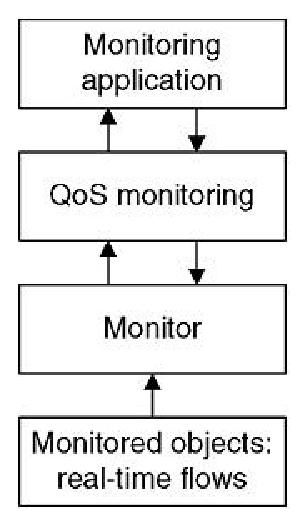
\includegraphics[width=0.3\textwidth]{modelo}
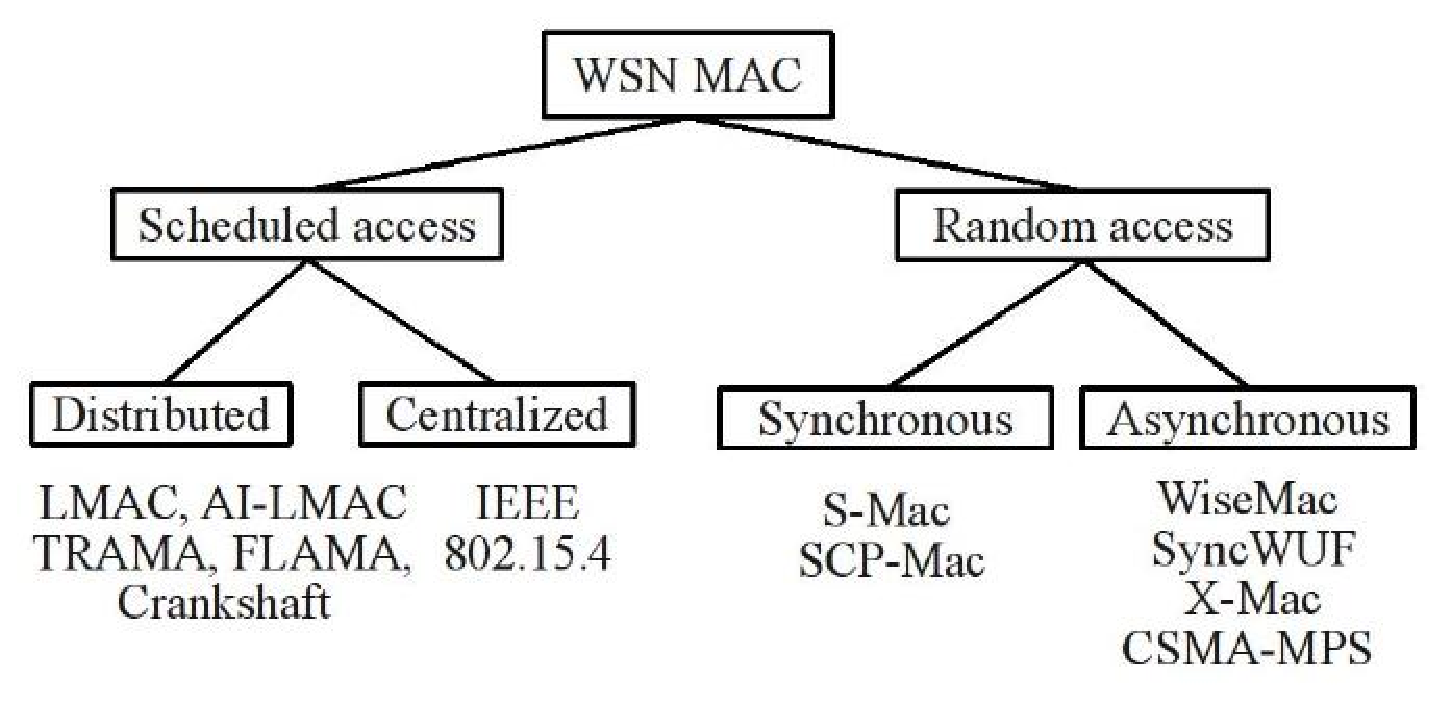
\includegraphics[scale=0.35]{imagens/classificacao}
\caption{Classificação das camadas MACs \cite{20085211817614}}
\label{fig:classicacao}
\end{figure}

  \subsection{PROTOCOLOS BASEADOS EM ESCALONAMENTO}
    Como já foi dito anteriormente, os protocolos baseados em escalonamento organizam o meio físico dividindo-o em slots, geralmente baseado na técnica de TDMA. Tradicionalmente, a opção por este tipo de protocolo pretende evitar problemas como \textit{idle listening}, \textit{overhearing} e colisões \cite{20100312645920}. Na verdade, a divisão em slots não implica que não ocorrerá colisões. Por exemplo, em \cite{20102813064978} a comunicação dentro de cada slot (que representa um \textit{cluster}) se dá através de contenção e em \cite{20083811560517} slots de dado (livre de contenção) podem se transformar em slots de controle (com contenção). 
    
    Nos dois casos acima, a colisão pode ocorrer pois estes protocolos são híbridos, ou seja, eles utilizam o melhor das técnicas com o intuito de criar um protocolo mais eficiente \cite{20092612148942}. Em alguns protocolos escalonados, apesar de estes possuirem um período em que o acesso é aleatório, os autores não deixam claro o por quê desta escolha, ou seja, é como se apenas fosse necessário para o funcionamento do protocolo. Neste caso, nós não consideramos híbrido.

    Os protocolos baseados em escalonamento são divididados em dois tipos: distribuído e centralizado.

  \subsubsection{Distribuído}
    os protocolos distribuídos híbridos \cite{20102813064978, 20102613043092, 20094012349418, 20093112234782, 20083811560517, 20092612148942, 20093812310584}, além dos \cite{20103113115754, 20100512680000}, são aqueles em que a tarefa de coordenação não é centralizada, ou seja, não existe um nó responsável por distribuir as mensagens de sincronização e definir o momento em que cada um deve se comunicar.

    Em \cite{20083811560517} é apresentado o protocolo híbrido \textit{Cooperative Wireless Sensor Medium Access Control} (CWS-MAC). Ele foi desenvolvido com o intuito de atender tanto aos requisitos das mensagens de controle como aos do tráfego dos dados. Diferente da forma como o tráfego das RSSF geralmente são caracterizadas, em \cite{20083811560517}, nas RSSF cooperativas, existem dois tipos de tráfegos: as mensagens de dado que são enviadas periodicamente e requisitam grande largura de banda (como multimídia), sendo estas tolerantes a descartes, e as mensagens de controle, sendo estas curtas, não tolerando descartes e necessitando o mínimo atraso. 
    
    As mensagens de dado são transmitidas de forma escalonada e sem colisão (os autores não apresentam o esquema de atribuição de slots, mas referenciam trabalhos), enquanto as mensagens de controle são transmitidas em mini-slots mas com contenção. Para garantir a confiabilidade, \textit{ACKs} são utilizados. Já para garantir o mínimo atraso, o CWS-MAC apresenta uma abordagem nova: o quadro de controle pode `roubar` o quadro de dado, ou seja, caso exista uma mensagem de controle pendente, esta terá prioridade sobre qualquer quadro de dado de qualquer nó, sobrepondo o quadro de dado com um quadro de controle.

    Nos resultados apresentados em \cite{20083811560517}, foram observados que a vazão não degrada com a saturação da rede e o atraso se mostrou menor se comparado às abordagens tradicionais de TDMA. É interessante observar que tipicamente em protocolos híbridos, utiliza-se a reserva para mensagens grandes e que necessitam de vazão, enquanto a contenção é reservada para as mensagens pequenas (de controle), cuja probabilidade de colidir é menor.

    %A MAC apresentada em \cite{20093812310584} é denominada \textit{Multi-Channel Flow-Aware Medium Access Control protocol} (MFLAMA).

  \subsubsection{Centralizado}
    Os protocolos centralizados híbridos \cite{20102613044996, 20092812183087}, além do \cite{20100312645920}, correspondem ao oposto dos protocolos distribuídos.

    O protocolo descrito em \cite{20100312645920} propõe a utilização de uma plataforma aérea de comunicação para auxiliar o trabalho da camada MAC, servindo como um coordenador central, eliminando a função de coordenação da RSSF, e/ou atuando como o próprio nó \textit{sink}. Como coordenador central, o dispositivo capturaria a informação de topologia de todos os nós e definiria o escalonamento de cada nó além de definir o melhor caminho a ser percorrrido por cada mensagem até o nó \textit{sink}, eliminando o protocolo de roteamento (consiste em uma solução \textit{cross-layer}, a ser detalhada posteriormente). Isto eliminaria a troca de mensagens de coordenação e roteamento. Atuando como nó \textit{sink}, a comunicação poderia ser direta, eliminando a comunicação \textit{multi-hop}. Figura \ref{fig:aerial} ilustra os dois casos.

    A motivação para a comunicação direta ao invés do caminho \textit{multi-hop} é que com um dispositivo aéreo a 200 metros de altura e os nós sensores com uma determinada angulação (da antena) e com uma certa frequência de interesse, seria possível haver comunicação direta com pouquíssima interferência do meio, ou seja, o modelo de decaimento do sinal \textit{free space} com uma fator de decaimento do sinal (característico do meio) de dois modelaria bem o efeito sobre o sinal. Enquanto isso, na comunicação terrestre, em decorrência à diversos efeitos, medidas mostram que o fator de decaimento fica entre três e quatro, ou seja, transmitindo uma mensagem com a mesma potência de transmissão nas duas situações, seria possível alcançar uma distância no ar muito maior se comparado com a comunicação terrestre.

    Para dar suporte às duas funcionalidades citadas anteriormente, são apresentados dois protocolos em \cite{20100312645920}: APRMAC e APMAC. O APRMAC é baseado no TRAMA \cite{rajendran03}, sendo responsável por definir o escalonamento de todos os nós, para que as mensagens sejam encaminhadas com o menor atraso possível. Os nós obtêm os vizinhos de um salto e enviam esta informação para o dispositivo. O APRMAC define para cada nó e em cada slot de tempo, o estado em que o nó deve estar: transmitindo, recebendo (para posteriormente encaminhar) ou dormindo. O APMAC é responsável por organizar para que cada nó transmita suas mensagens, livre de colisão, para o dispositivo aéreo, sendo que o protocolo se adapta ao tráfego.
    
\begin{figure}
\centering
%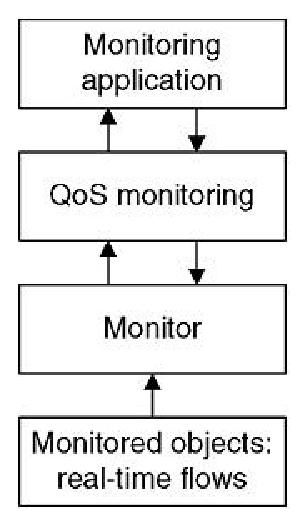
\includegraphics[width=0.3\textwidth]{modelo}
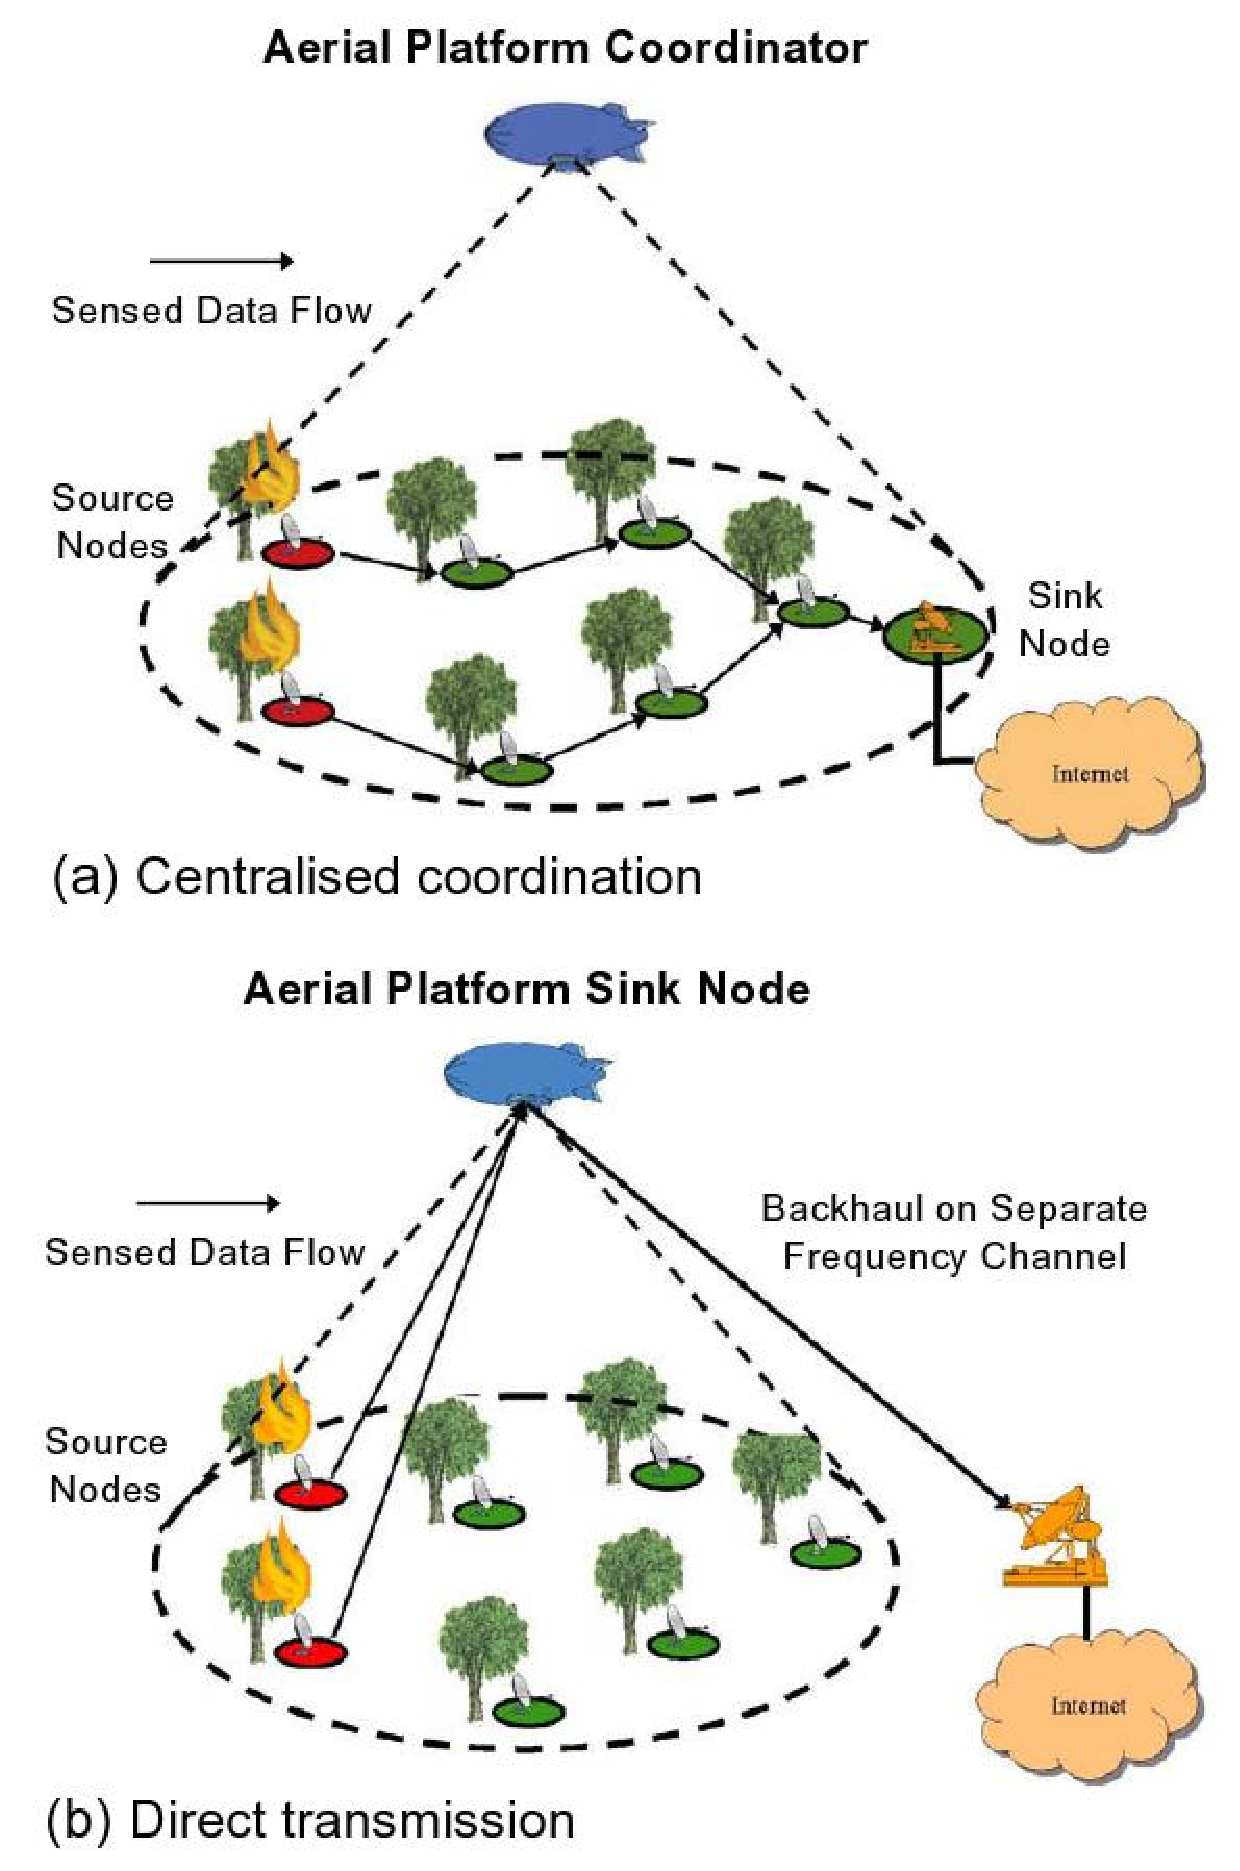
\includegraphics[scale=0.25]{imagens/aerial}
\caption{Suporte aéreo para protocolo MAC \cite{20100312645920}}
\label{fig:aerial}
\end{figure}

  \subsection{PROTOCOLOS DE ACESSO ALEATÓRIO}
    Como já foi dito, nos protocolos de acesso aleatório, o acesso não é regulado e ocorre sob-demanda. Neste tipo de protocolo, um dos principais benefícios consiste na extensibilidade \cite{20100312645920}, visto que \textit{overhead} de coordenação não existe, diminuindo inclusive o gasto energético em decorrência disso. Entretanto, ela sofre com \textit{idle listening}, \textit{overhearing} e colisão.

    Como já foi dito, \emph{overhearing} consiste em uma das principais formas de gasto energético em RSSF. Muitos protocolos estão sujeitos ao \emph{overhearing}. Todos os protocolos que se baseiam na técnica denominada 
\emph{low power listening} (LPL), também conhecida por amostragem de preâmbulo (\emph{preamble sampling}) \cite{Polastre04, Hoiydi04, Buettner06, 20100312644073, 20103113115841}, estão sujeitos 
ao efeito do \emph{overhearing}, basicamente pelo fato de serem protocolos assíncronos. Em particular, B-MAC \cite{Polastre04}, um protocolo baseado em amostragem de preâmbulo, consiste 
no protocolo padrão para o \emph{TinyOS} \cite{Buettner06}, um dos sistemas operacionais mais importantes para RSSF. Além disso, o protocolo para MAC especificado no padrão IEEE 802.15.4 \cite{Society2006}, o padrão 
\emph{de facto} para camada MAC e física para dispositivos de baixo consumo, está sujeito ao \emph{overhearing}.

    Os protocolos de acesso aleatório podem ser divididos em: síncrono e assíncrono.
  
  \subsubsection{Síncrono}
    Nos protocolos síncronos  \cite{20064010146973, 20102012936055, Yadav08, 20100812725891, 20101312811704}, mecanismos de sincronização entre os nós são adotados. Geralmente, esta sincronização proporciona aos nós tomarem conhecimento dos escalonamentos dos vizinhos, objetivando reduzir o \textit{idle listening}.

    Em \cite{Yadav08}, é proposto um protocolo que consiste numa variação do S-MAC \cite{Wei02} além de conter algumas otimizações. O protocolo tem por objetivo a eficiência energética e latência, baseado nas limitaçãoes do S-MAC e T-MAC \cite{Dam03}. 

    A sincronização dos nós é semelhante ao S-MAC. Os endereços de origem e destino foram removidos das mensagens de dado. Além disso, as mensagens de sincronização e de RTS foram convertidas em um único pacote de controle. Tudo isso com o intuito de diminuir o \textit{overhead}, consequentemente diminuindo o atraso. Diferente do S-MAC, o nó se adapta ao tráfego variando o \textit{duty cycle}. 
O \emph{duty cycle} consiste em, para cada ciclo de operação, a relação entre o tempo que o nó permanece acordado pelo tempo total do ciclo. Quando a quantidade de pacotes na fila é maior que um limite, o \textit{duty cycle} é incrementado (por um fator de dois). Quando está abaixo de um limite, é decrementado (também por um fator de dois).

    Em \cite{20102012936055}, também é proposta uma variação do S-MAC. O objetivo dos autores é reduzir o \textit{idle listening} do S-MAC. Para isso, o protocolo varia o tamanho da janela de contenção (\textit{Contention Window} - CW) dependendo do tráfego. A quantidade de tráfego é percebida através das trocas de RTS e CTS, dando indício da possível quantidade de nós que irão futuramente participar da contenção. O tráfego é estimado a partir do número de colisões, tamanho médio das colisões e tamanho médio dos tempos no estado ocioso. 

    A lógica para calcular o CW consiste no seguinte: à medida em que o tráfego torna-se menos intenso, a probabilidade de colisão é menor, logo o valor do CW pode ser menor, reduzindo energia. Caso o tráfego aumente, aumenta-se o CW, fazendo com que a colisão diminuia. Observe que apesar de ajustar o CW a partir do tráfego, o protocolo não se adapta ao tráfego, pois o \textit{duty cycle} continua fixo.

    %logica fuzzy \cite{20101312811704, 20100812725891}
    %20101312811704 eh baseada em cluster

  \subsubsection{Assíncrono}

    O protocolo \textit{Game-theoretic} (G-MAC) é apresentado em \cite{20093112234782}. Assim como o CWS-MAC, o G-MAC tem por fim garantir vazão e mínimo atraso (outros protocolos que também consideram QoS como objetivo final serão apresentados na Seção IV). A motivação do trabalho consiste no fato de que as aplicações estão começando a ter requisitos de tempo-real. Em \cite{20093112234782}, o autor tenta otimizar vazão e atraso levando em consideração as restrições energéticas. 

    O autor modela como um problema de otimização com restrição baseado em um jogo (\textit{Teoria dos Jogos}) cooperativo incompleto. O autor modela como um jogo, pois há uma situação de conflito (entre energia e requisitos de QoS), além de haver cooperação, que neste caso é incompleta. O jogo é considerado incompleto pois a estratégia de cada jogador é tomada baseada no estado dos outros jogadores sem haver troca de estados. Esta é uma inovação do trabalho. Além disso, o problema foi modelado com restrições energéticas, diferentemente de trabalhos anteriores. A estratégia de equilíbrio de cada jogador consiste em três ações: transmitir, escutar ou dormir. O autor propõe uma heurística que, para cada estado corrente do jogo, calcula o tempo no estado ativo, o tempo no estado inativo (\textit{sleep}) e a probabilidade de enviar uma mensagem, caso esteja no estado ativo. O autor definiu como sendo o estado do jogo a quantidade de nós disputando o acesso ao meio, sendo que esta quantidade é estimada através da probabilidade de transmitir e de colisão.

    Por fim, em \cite{20093112234782} é proposto o G-MAC. Neste protocolo, o tempo é dividido em super-quadros, formados por duas partes: ativa e inativa. O tamanho destas duas partes é ajustada pela estratégia de equilíbrio de cada jogador. O acesso na parte ativa é feita de forma aleatória e alguns parâmetros da contenção, como o tamanho da janela de \textit{backoff}, são ajustados também pela estratégia de equilíbrio. Nos resultados obtidos, G-MAC se mostrou melhor em termos de vazão e latência quando comparado com S-MAC e T-MAC, enquanto a energia consumida foi considerada pelo autor relativamente baixa.

  \subsection{Protocolos Multicanais}
    Os protocolos multicanais \cite{20084511683228, 20093812310584, 20083911592812} são aqueles que utilizam mais de um canal para transmitirem as mensagens de controle e de dados.
  
    Em \cite{20084511683228}, a motivação para o trabalho é que, com o avanço do \textit{hardware}, nós sensores agora podem se comunicar em mais de um canal. Dado isso, há a necessidade de utilizar os canais de comunicação que provoquem o mínimo de interferência possível. Este problema equivale ao problema de colorir em grafos, onde cores que separam nós com até dois saltos de distância devem ser diferentes. Eles propõem uma heurística para resolver este problema, denominada \emph{Alocação Dinâmica de Canal} (\textit{Dynamic Channel Allocation} - DCA).

    Além do DCA, em \cite{20084511683228} é proposto um protocolo multicanal, o CMAC. O objetivo principal de CMAC é conservar energia. No desenvolvimento do protocolo, eles objetivaram reduzir o \textit{idle listening}, visto que este corresponde à principal fonte de gasto energético \cite{Reason04}. Eles pressupõem que o sensor é equipado com dois tipos de transceptores (rádios): um com funções reduzidas (o LR) e um mais robusto (MR) capaz de transmitir em qualquer canal (dentro do conjunto definido). Além disso, assumem que o \emph{MR} transmite à potência constante (inviabiliza o uso de controle de topologia). Este rádio é responsável pela transmissão dos dados. O \emph{LR} consiste em um rádio de menor potência (\textit{low-power radio}), sendo este responsável por emitir e receber sequências de pulsos que codificam as mensagens de controle.

    No protocolo, existem três tipos de mensagens: \textit{REQ}, \textit{CON} e \textit{WAIT}. A comunicação ocorre em duas fases: fase de negociação e a fase da comunicação do dado. Quando um nó \emph{S} deseja enviar uma mensagem para \emph{R}, o \emph{LR} de \emph{R} monitora o canal de \emph{S} e, caso este esteja livre (o procedimento de \emph{backoff} e de prevenção de colisão do 802.11 é adotado), LR de \emph{R} transmite \emph{REQ} no canal de \emph{S}, sendo que \emph{REQ} identifica o canal de \emph{R}. Figure \ref{fig:cmac} ilustra a troca de mensagens. Caso o canal de \emph{S} esteja livre, \emph{S} envia no seu próprio canal a mensagem de \emph{CON}, sendo que esta identifica o canal de \emph{S}. Isto é necessário para identificar o vencedor, caso haja mais de um concorrente. Caso o canal estivesse ocupado, \emph{S} receberia um \emph{WAIT} que identificaria por quanto tempo ele deve aguardar até a comunicação finalizar. Caso \emph{S} receba \emph{CON}, \emph{MR} de \emph{S} será ligado e a fase de tranmissão do dado iniciará no canal de \emph{S}. Observe que \emph{MR} de \emph{R} também deverá ligar e mudar para o canal de \emph{S}. Ao fim da comunicação, um \emph{ACK} é enviado pelo \emph{MR} de \emph{R} no canal de \emph{R}, ou seja, \emph{S} deve aguardar o \emph{ACK} no canal de \emph{R}.

    Ainda em \cite{20084511683228}, os autores justificam a necessidade desta última troca de canal, além de mostrar como colisões e \textit{overhearing} são tratados. A comunicação do dado útil é livre de colisão. Resultados mostram que quando comparado com o S-MAC, CMAC obtém significativa redução do consumo de energia e de atraso além do aumento da vazão.

    %observe que não vai haver problema de interferÊncia

\begin{figure}
\centering
%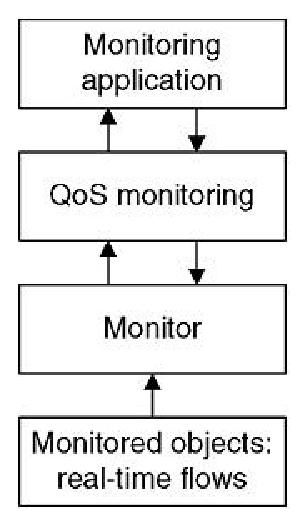
\includegraphics[width=0.3\textwidth]{modelo}
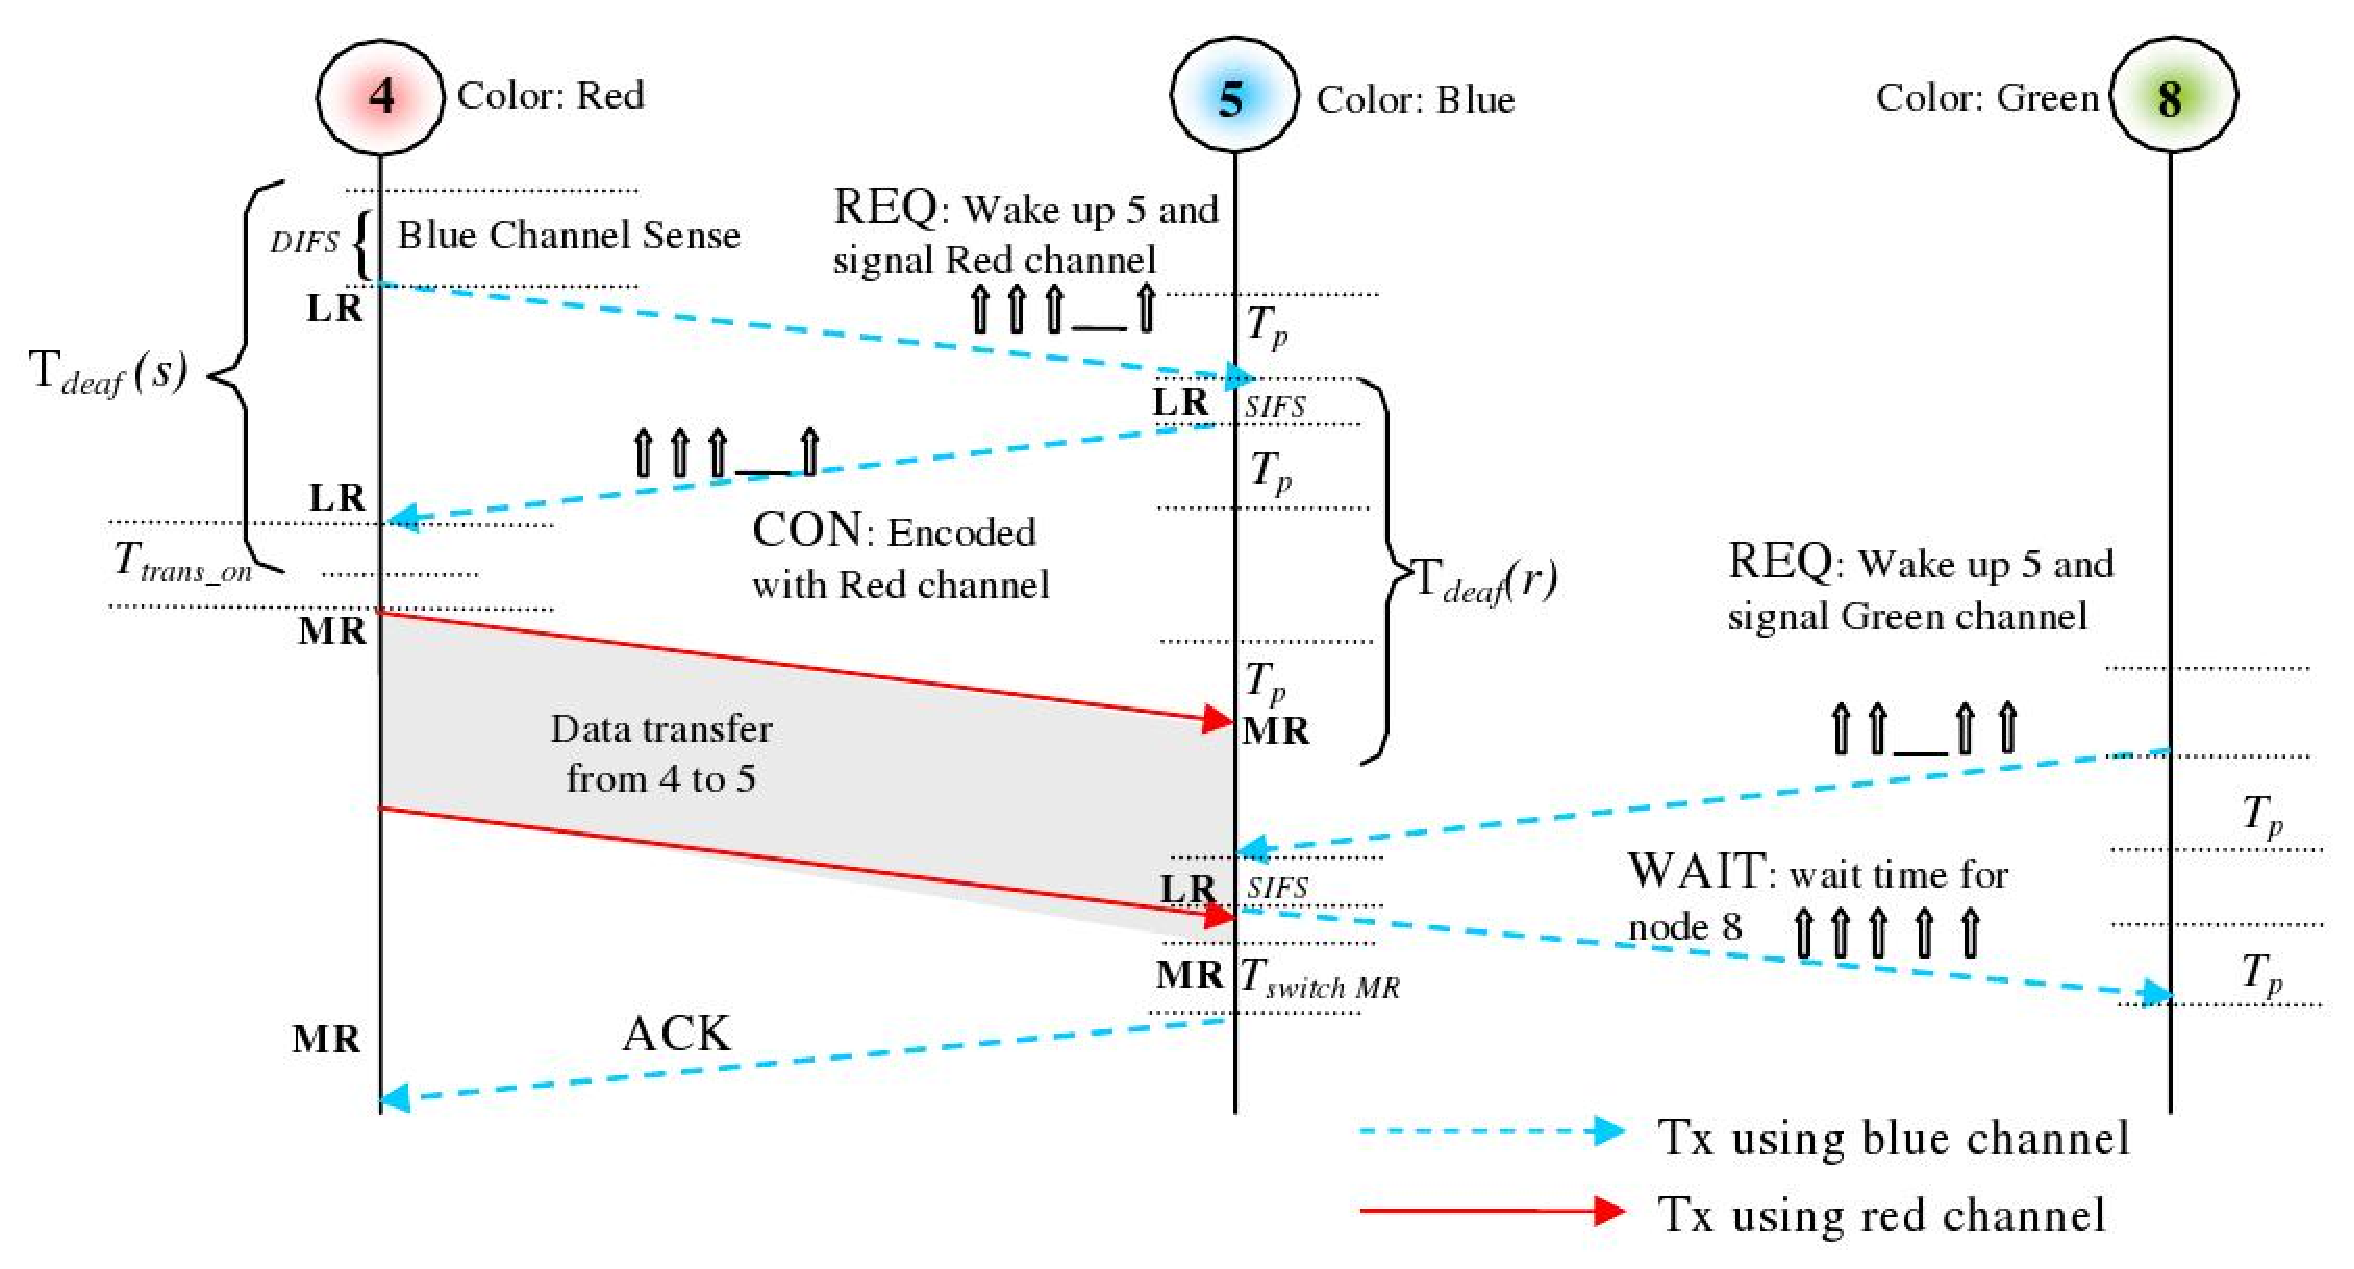
\includegraphics[scale=0.20]{imagens/cmac}
\caption{Troca de mensagens no CMAC \cite{20084511683228}}
\label{fig:cmac}
\end{figure}    
  
  \section{CARACTERÍSTICAS}
  \label{caracteristicas}
  Nos trabalhos mais recentes, alguns trabalhos apresentam características interessantes que os diferem dos demais. Estas características são: suporte à mobilidade, \emph{design cross-layer},
protocolos baseados em modelo de controle de potência e dinamicidade.

  \subsection{MOBILIDADE}
    Apenas um protocolo foi encontrado que fornece suporte à mobilidade \cite{20103113115754}. Em \cite{20100312645920}, os autores apenas mencionam que o suporte à mobilidade é fornecido diminuindo o tamanho do quadro (reduzindo o tempo do ciclo) para que atualizações frequentes possam ocorrer.
    %trabalhos futuros que visam fornecer suporte à mobilidade
    
    O protocolo apresentado em \cite{20103113115754} é inovador no que se refere à capacidade de fornecer suporte à mobilidade de um \textit{cluster} de nós. Além da própria movimentação dos \textit{clusters}, existe ainda a possibilidade de movimentação individual dos nós dentro do \textit{cluster}. Os autores categorizam os nós sensores em dois tipos: nós \textit{estáticos}, que podem se mover de forma bastante limitada, e os nós \textit{móveis}.

    Na motivação para o trabalho, os autores dão destaque às aplicações ligadas à área de saúde, como por exemplo aplicações para monitorar o estado de saúde de pessoas idosas. Um tipo de rede com esta característica é a \textit{Wireless Body Area Network} (WBAN). Este tipo de aplicação é caracterizado pela movimentação de \textit{cluster} de nós. Nas WBANs, um conjunto de nós sensores são posicionados ao longo do corpo do paciente para sensoriar e atuar de diversas formas. O consumo energético dos nós da WBAN deve ser muito baixo. Neste tipo de cenário, em complemento às WBANs, existem também as redes fixas. Os nós das redes fixas se comunicam com as WBANs tanto para capturar informação como para passar informação. Tipicamente neste cenário, os protocolos de roteamento são baseados em \textit{gossiping}. Este tipo de técnica visa a confiabilidade pois as mensagens são transmitidas com redundância.

    Para dar suporte à mobilidade, é importante adotar um modelo de mobilidade, pois este tenta capturar o padrão de movimentação dos sensores. Em \cite{20103113115754}, eles comentam sobre o modelo adotado.

    Em \cite{20103113115754}, os autores propuseram o \textit{Mobile Cluster MAC} (MCMAC), sendo este baseado em um outro protocolo que dá suporte à técnica de \textit{gossiping}. No MCMAC, os autores incorporaram a característica de mobilidade dos nós.

    No MCMAC, o quadro é dividido em duas partes: ativo e inativo. Este quado se assemelha ao quadro do GMAC, protocolo do qual ele retirou esta estrutura. Figura \ref{fig:mcmac} ilustra o quadro do MCMAC. A primeira parte dos slots ativos (\textit{Static Active Slots} - SAS) são utilizados pelos nós estáticos para comunicarem entre si. Esta parte foi herdada do GMAC. A segunda parte ativa é conhecida como \textit{mobile cluster slots} (MCS) sendo utilizada pelos nós móveis. Assim como no SAS, no MCS deve-se garantir que cada slot seja atribuído a apenas um nó. 

    Para os nós estáticos receberem mensagens dos nós móveis, eles precisam escutar durante o MCS, e para os nós móveis receberem mensagens dos nós estáticos, eles precisam escutar o SAS. Quando um \textit{cluster} está próximo de outro, pode ocorrer colisão (devido à sobreposição). Eles resolvem isso adicionando o CSMA dentro de cada slot, como está ilustrado na Figura \ref{fig:mcmac}.

    Os autores também propõem várias otimizações com o intuito de reduzir o consumo energético.
    
\begin{figure}
\centering
%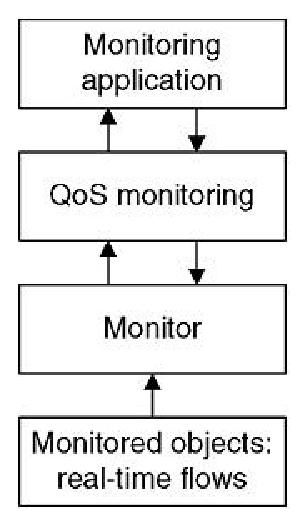
\includegraphics[width=0.3\textwidth]{modelo}
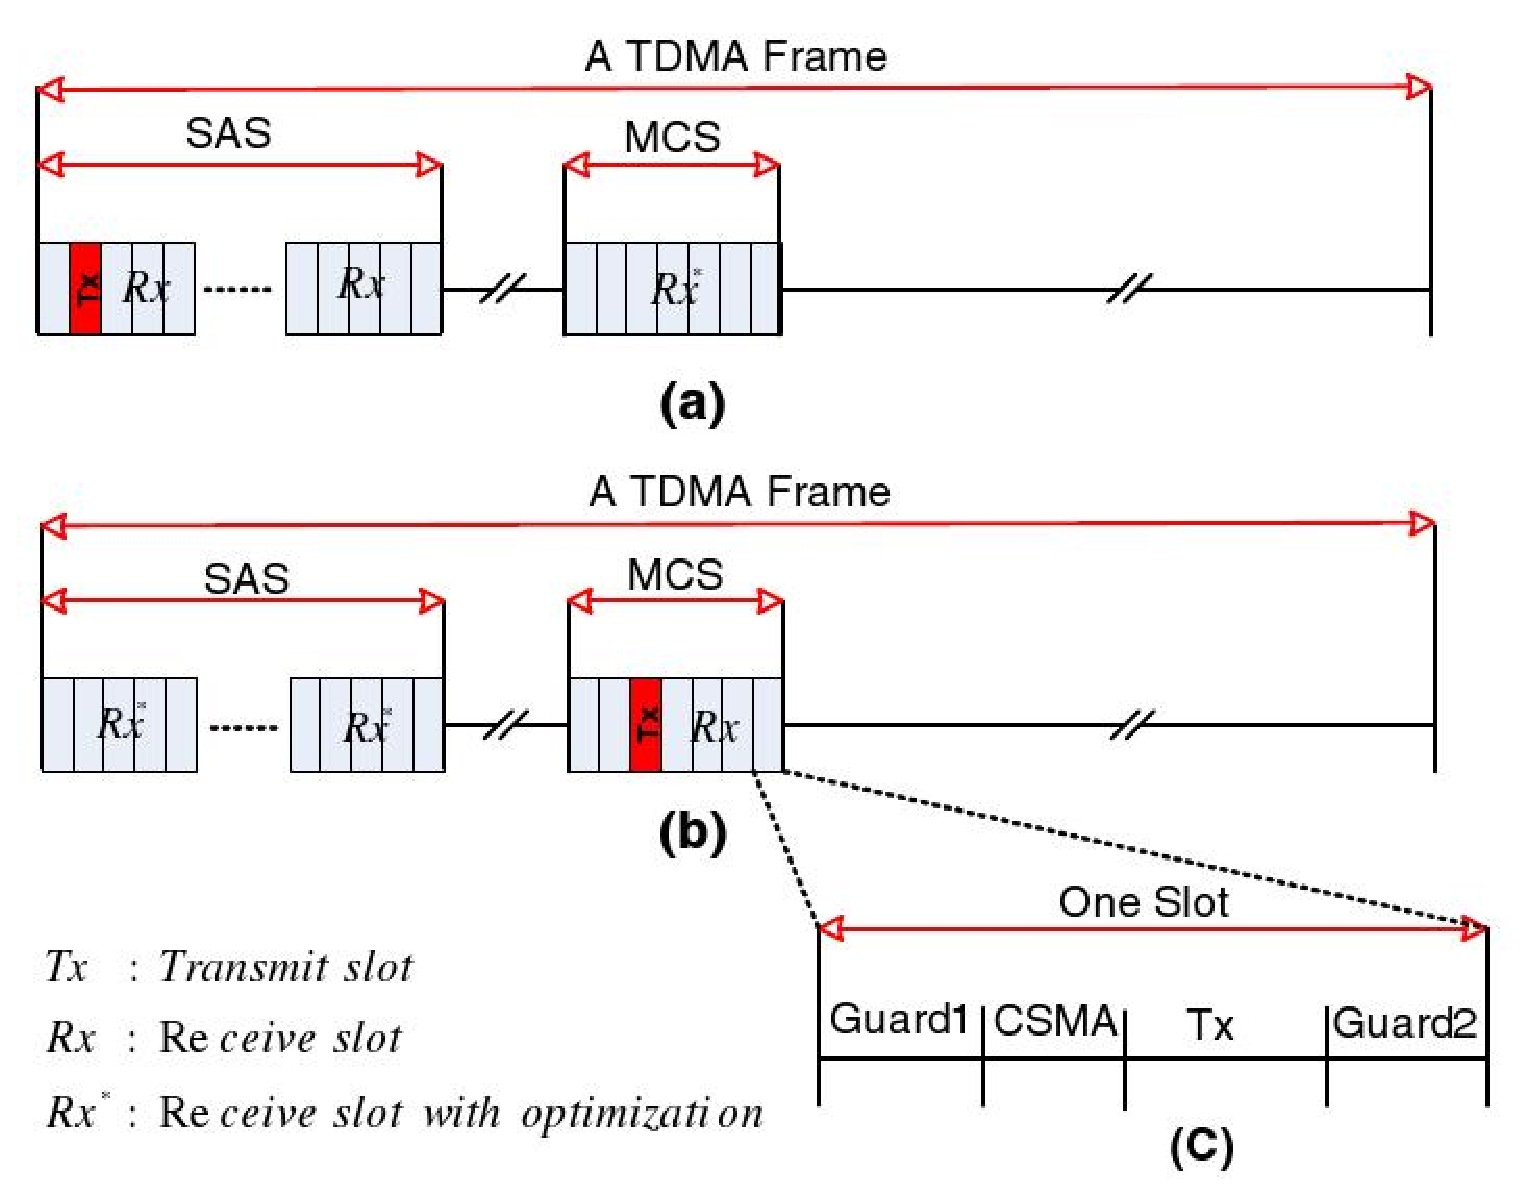
\includegraphics[scale=0.35]{imagens/mcmac}
\caption{Frame do MCMAC \cite{20103113115754}}
\label{fig:mcmac}
\end{figure}

  \subsection{DESIGN CROSS-LAYER}
    Alguns protocolos possuem a característica de extrapolar a região que lhe concerne. Em alguns protocolos como em \cite{20083811560517, 20092612148942}, para que seja possível priorizar uma classe de tráfego, é necessário ter conhecimento da prioridade dos mesmos, que é definida pela aplicação. Em outros casos, o protocolo elimina a camada de roteamento, seja porque ele mesmo realiza esta função \cite{20100312645920} ou porque força uma determinada topologia na rede, eliminando a necessidade de decisão por parte do roteamento \cite{20092812183087, 20093812310584}.

    Em \cite {20092812183087} é proposto o protocolo MaCARI, que faz parte de um outro projeto citado em \cite{20092812183087}. MaCARI consiste em um protocolo híbrido, onde seu período é dividido em três partes: sincronização, um período escalonado que está relacionado com a ávore que representa a topologia da RSSF, ou seja, a comunicação entre os nós segue uma estrutura fixa e, por último, um período não escalonado.
    
    No período de sincronização, todos os nós da árvore necessitam ser sincronizados, ou seja, requer sincronização global. No período escalonado, o acesso ao meio é feito livre de colisão. Cada nó da árvore que possui um filho é considerado um coordenador, sendo que o período escalonado, para o coordenador, é dividido em duas partes: uma para se comunicar com os nós filhos que não são coordenadores e outra para se comunicar com os nós coordenadores com os quais possui algum vínculo na árvore. Já no período não escalonado, cada coordenador pode se comunicar com qualquer outro coordenador ao seu alcance, utilizando CSMA/CA.

  \subsection{PROTOCOLOS COM CONTROLE DE POTêNCIA}
    Em \cite{20094212373426} é apresentada C-MAC, um protocolo que tenta explorar o fato que transmissões concorrentes, ou seja, transmissões que interferem umas nas outras, podem ser realizadas com sucesso. O autor mostra um exemplo com dois enlaces de comunicação, sendo que um interfere no outro, e foi visto que a vazão é maior quando o CSMA não está habilitado, ou seja, há a possibilidade de comunicação mesmo quando enlaces interferem uns com os outros.

    Modelos de interferência são estudados em \cite{20094212373426} e os autores mostram que existe uma relação entre a razão de recebimento de pacote (\textit{Packet Reception Ratio} - PRR) e o SINR (\textit{Signal-to-Interference-plus-Noise-Ratio}). O objetivo da C-MAC é maximizar a vazão mesmo na presença de interferência, desabilitando totalmente o CSMA. A partir da relação PRR-SINR, C-MAC tenta estimar qual o melhor momento e a melhor potência de transmissão para que a vazão possa ser maximizada.

    Uma das vantagens do trabalho é que os modelos adotados são empíricos ao invés de modelos simplistas que assumem que a atenuação da potência é simétrica. Resultados mostraram que, comparado com outros protocolos baseados em CSMA, o C-MAC conseguiu resultados melhores em termos de vazão, atraso e consumo de energia.

  \subsection{DINAMICIDADE}
    Algumas protocolos têm a capacidade de variar o \textit{duty cycle} e/ou o tempo do ciclo do quadro com intuito de se adaptar ao tráfego \cite{20064010146973, 20102613044996, Yadav08, 20100512680000, 20093112234782, 20101312811704}. Isto permite o aumento da vazão, assim como a redução do atraso. O consumo energético também tende a diminuir, pois o \textit{idle listening} é reduzido.

    Em \cite {20100812725891} é proposto um protocolo denominado \textit{Fuzzy Logic-based Adaptative Listen for Medium Access Control} (FLAMAC) que tem por fim a redução do consumo energético através da redução do \textit{idle listening}. Diferente das outras MACs deste grupo, FLAMAC reduz o \textit{idle listening} variando o tempo do ciclo do quadro ao invés do \textit{duty cycle}, sendo que este último fica fixo. O protocolo, como o próprio nome diz, é baseado em logica \textit{fuzzy}, pois os autores consideram esta técnica versátil e que requer baixo poder computacional, sendo adequada para as RSSF. Além disso, eles utilizam lógica \textit{fuzzy} pois acreditam que o problema consiste em um sistema de controle que identifica a energia corrente e o tráfego atual e toma a decisão para mudar o tempo do ciclo.

   Lógica \textit{fuzzy} também é adotada em \cite{20101312811704}. Neste trabalho, os autores adotam \textit{fuzzy} para ajustar o momento em que a difusão de mensagens de escalonamento deve ocorrer. Quando muitas mensagens estão sendo perdidas em decorrência do desvio dos relógios ou pelo fato de os tempos do estado ativo e inativo terem sido mal escolhidos, é necessário encurtar a periodicidade de divulgação do escalonamento. Caso contrário, a periodicidade deve ser aumentada. Desta forma, através da lógica \textit{fuzzy}, o overhead das mensagens de escalonamento é gerado na medida adequada.  

  \section{MÉTRICAS VISADAS}
  \label{metricas}

  Como já foi dito anteriormente, nos últimos anos, além da redução do consumo energético, outras métricas têm sido priorizadas pelos pesquisadores na elaboração dos protocolos, dentre elas vazão, atraso e aumento da razão de entrega de mensagens. Muitos trabalhos buscam melhorar estas métricas mas não as colocam como objetivos principais. Isto pode ser visto, com relação ao atraso, em \cite{20083811569004, 20102012936055, 20101312811704}. Muitos trabalhos colocam o atraso e/ou vazão como objetivos principais, no mesmo patamar ou acima da redução de gasto energético, objetivando garantir \textit{Qualidade de Serviço} \cite{20064010146973, 20102613043092, 20093112234782, 20093812310364, 20083811560517, 20083811569004, 20092612148942}.

  Em \cite{20092612148942} é apresentado o EQ-MAC, um protocolo que tem por objetivo prover Qualidade de Serviço através dos \textit{Serviços Diferenciados}, ao passo que reduz energia. EQ-MAC é formada por dois componentes: \textit{Classifier MAC} (C-MAC) e \textit{Channel Access MAC} (CA-MAC).

  C-MAC é responsável por fazer a classificação do tráfego para que o mesmo possa ser tratado de forma diferenciada. $\CMAC$ requer que a camada de aplicação indique a prioridade do dado no cabeçalho do mesmo, para que cada pacote de dado seja encaminhado para uma fila diferente. Figura \ref{fig:eq-mac} ilustra o C-MAC e a estrutura do EQ-MAC como um todo.

  O EQ-MAC consiste em um protocolo híbrido, utilizando o acesso aleatório para as mensagens de controle e o período escalonado para as mensagens de dado. Para o CA-MAC, existem dois tipos de nós: os nós comuns e os chefes (\textit{heads}). O \textit{head} é responsável pela função de coordenação. Cada quadro do CA-MAC é formado por duas partes: \emph{mini slot} e \emph{slot normal}. Os mini slots servem para transmitir mensagens de controle enquanto os slots normais transmitem dados. A comunicação ocorre em quatro fases, sendo estas necessárias para que os nós normais possam requisitar slots de dado, informando a prioridade das mensagens que os mesmos possuem, para que então o \textit{head} possa alocar os slots de dado para estes nós, levando em consideração a prioridade das mensagens.

  O trabalho de \cite{20102613043092} consiste numa continuidade e melhora do trabalho em \cite{20092612148942}.

\begin{figure}
\centering
%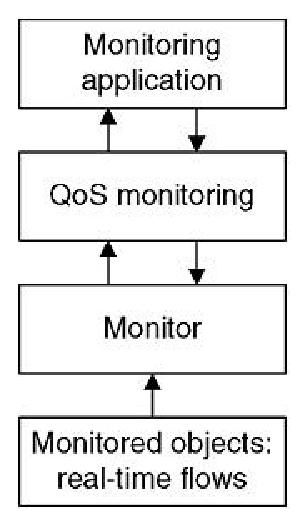
\includegraphics[width=0.3\textwidth]{modelo}
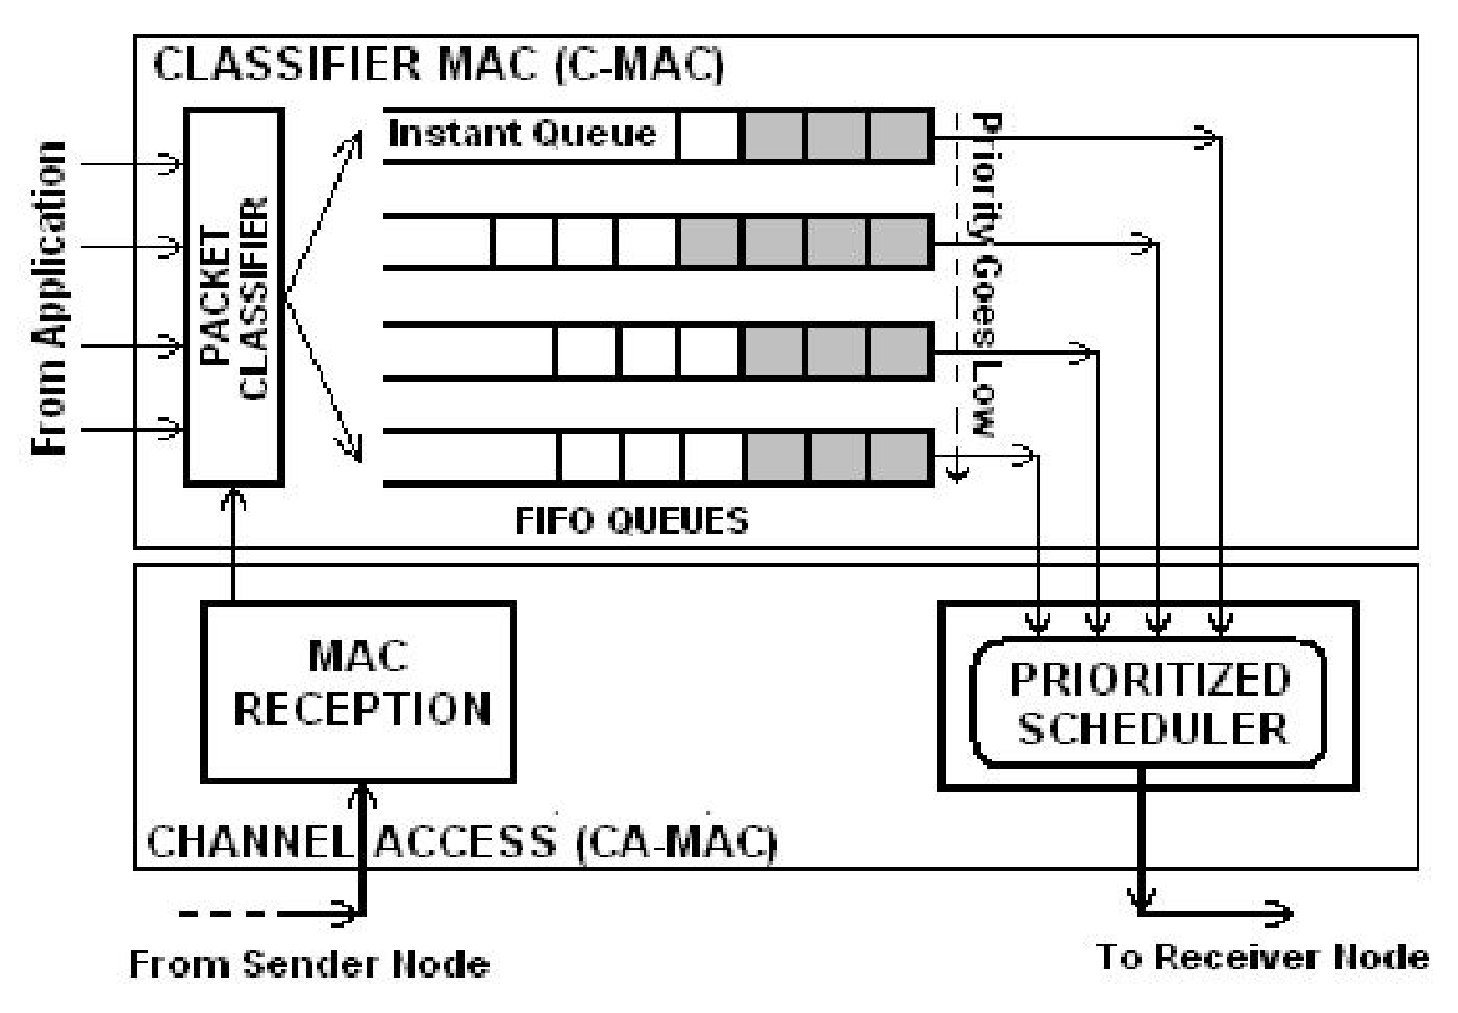
\includegraphics[scale=0.35]{imagens/eq-mac}
\caption{Estrutura do EQ-MAC \cite{20092612148942}}
\label{fig:eq-mac}
\end{figure}

  \section{CONSIDERAÇÕES FINAIS}
  \label{final}

  Os protocolos para MAC continuam sendo bastante pesquisadas em RSSF principalmente por serem a principal forma de interferir no consumo energético. Além disso, em decorrência da peculiaridade de cada aplicação, não existe uma camada padrão, fazendo com que objetivos diferentes sejam visados pelos pesquisadores.

  Os protocolos têm optado por soluções híbridas, objetivando reunir o melhor das duas técnicas, ou melhor, utilizando cada uma no momento adequado ou para o elemento adequado (por exemplo, o tipo de tráfego).

  Quando existe mais de um objetivo ao mesmo tempo, ou seja, uma solução de compromisso deve existir, técnicas como lógica \textit{fuzzy} e Teoria dos Jogos têm sido adotados.

  Os protocolos também têm relevado adaptação ao tráfego, seja variando o \textit{duty cycle}, seja variando o tempo do ciclo do quadro.

  A adoção de mais de um canal de comunicação tem surgido, assim como \textit{design cross-layer}. Outra característica interessante são os protocolos que assumem que é possível haver comunicação mesmo na presença de interferência.

  O suporte à mobilidade não tem sido incorporado à grande maioria dos protocolos. Este suporte passa a ser necessário em redes WBAN.

  Muitos trabalhos têm por fim a obtenção de Qualidade de Serviço (representado pela reunião das métricas de vazão e atraso). QoS deixa de ser objetivo secundário à medida que novas aplicações vão surgindo (multimídia, sistemas com restrições temporais).
  %qos e outra metricas

\bibliographystyle{sbc}
\bibliography{macs}
\end{document}